\section{Results}
\label{sec:results}

We answer five questions.
\begin{itemize}
\item \RQ{1}: How often do detectors flag benign agent tool outputs, and how many agent tasks does that stop?
\item \RQ{2}: How many injections do detectors catch at 1\% FPR, and does a detector's rank on one benchmark predict its rank on another?
\item \RQ{3}: Does what a detector was trained on explain where it works?
\item \RQ{4}: Does knowing the user's request help, and which attack goals does each approach miss?
\item \RQ{5}: Do input format and metadata change false positives?
\end{itemize}

\begin{table*}[t]
\centering\small
\caption{All detectors on all sets. General: README, email, and web text. FPR at each detector's default threshold on benign tool outputs (AD-Clean, TB-Clean); ``tasks'' is the share of tasks with at least one flagged benign output. TPR at the threshold that gives 1\% FPR on the same set. BIPIA uses test-half attacks. ``Agent data'': the model card states training on agent or tool-output inputs; ``eval.'' means the card reports evaluation on AgentDojo-derived data. $^\dagger$Undocumented use of Sheltron's user-goal segment. Bootstrap intervals for four methods are in Appendix Table~\ref{tab:main}.}
\label{tab:many}
\resizebox{\textwidth}{!}{% generated by analysis/compute_many.py
\begin{tabular}{@{}lccc|c|cc|cc|ccc|c@{}}
\toprule
 & & & & General & \multicolumn{4}{c|}{AgentDojo} & \multicolumn{3}{c|}{$\tau$-bench} & BIPIA \\
 & & & Agent & FPR & FPR & Tasks & \multicolumn{2}{c|}{TPR @ 1\% FPR} & FPR & Tasks & TPR & TPR \\
Detector & Year & Size & data & (\%) & (\%) & (\%) & Matched & Shift & (\%) & (\%) & @ 1\% & @ 1\% \\
\midrule
JasperLS & 2023 & 184M & no & 99.9 & 78.5 & 97.9 & 23.4 & 22.1 & 93.1 & 99.6 & 18.7 & 4.9 \\
ProtectAI v1 & 2023 & 184M & no & 0.3 & 3.5 & 12.4 & 0.7 & 7.5 & 5.1 & 6.8 & 23.3 & 0.4 \\
ProtectAI v2 & 2024 & 184M & no & 3.8 & 30.1 & 69.1 & 0.5 & 0.8 & 66.9 & 80.3 & 10.1 & 0.7 \\
ProtectAI v2-small & 2024 & 142M & no & 1.6 & 12.1 & 34.0 & 7.6 & 3.1 & 1.4 & 2.8 & 30.1 & 1.4 \\
TestSavant-L & 2024 & 184M & no & 3.8 & 3.2 & 10.3 & 27.8 & 24.7 & 1.8 & 3.4 & 24.5 & 16.3 \\
Prompt Guard 1 & 2024 & 279M & no & 5.8 & 31.9 & 53.6 & 9.5 & 1.5 & 4.8 & 9.3 & 2.9 & 36.0 \\
PIGuard & 2025 & 184M & no & 9.4 & 29.5 & 59.8 & 2.1 & 7.9 & 11.0 & 20.9 & 52.7 & 95.1 \\
Prompt Guard 2 (22M) & 2025 & 71M & no & 0.3 & 0.0 & 0.0 & 60.9 & 63.6 & 0.0 & 0.0 & 60.8 & 31.7 \\
Prompt Guard 2 (86M) & 2025 & 279M & no & 0.1 & 0.6 & 2.1 & 69.4 & 78.8 & 0.0 & 0.0 & 57.9 & 10.4 \\
Qualifire Sentinel & 2025 & 396M & no & 18.2 & 0.9 & 3.1 & 61.1 & 66.4 & 0.0 & 0.0 & 21.9 & 4.6 \\
Sentinel v2 & 2025 & 596M & no & 17.2 & 2.1 & 7.2 & 20.8 & 16.5 & 0.5 & 1.2 & 68.7 & 20.2 \\
Sheltron & 2026 & 68M & yes & 12.0 & 10.6 & 28.9 & 20.1 & 26.4 & 4.4 & 6.7 & 95.2 & 57.2 \\
Sheltron (+task)$^\dagger$ & 2026 & 68M & yes & 12.0 & 26.0 & 47.4 & 9.0 & 18.8 & 69.7 & 85.0 & 65.4 & 8.0 \\
Prismor-1.5B & 2026 & 1.5B & no & 57.7 & 6.5 & 17.5 & 72.2 & 79.4 & 46.2 & 67.7 & 15.2 & 4.0 \\
Wolf Defender & 2026 & 308M & eval. & 3.1 & 0.9 & 3.1 & 73.8 & 83.9 & 0.0 & 0.0 & 90.8 & 3.5 \\
Horizon-Labs & 2026 & 308M & yes & 1.1 & 0.0 & 0.0 & 82.2 & 87.9 & 0.7 & 1.6 & 100.0 & 37.7 \\
\midrule
Judge (Qwen2.5-7B) & -- & 7B & -- & -- & -- & -- & 57.4 & 64.4 & 4.4 & 9.0 & 54.3 & 14.9 \\
Judge (Llama-3.1-8B) & -- & 8B & -- & -- & -- & -- & 55.3 & 61.9 & 5.4 & 9.6 & 78.3 & 8.3 \\
\bottomrule
\end{tabular}
}
\end{table*}

\subsection{RQ1: False Positives on Benign Tool Outputs}
\label{sec:rq1}

False alarms on benign tool outputs vary from none to most (Table~\ref{tab:many}). On AgentDojo, Horizon-Labs flags \MHZClean of AD-Clean outputs and Wolf Defender \MWFClean; they would stop \MHZBlock and \MWFBlock of tasks. ProtectAI v2 and PIGuard flag \CleanPAFPR and \CleanPGFPR of outputs and would stop \CleanPABlock and \CleanPGBlock of tasks (95\% intervals \CleanPABlockCI{} and \CleanPGBlockCI{}). Both Prompt Guard~2 models flag \MPGtClean and \MPGtsClean. On $\tau$-bench's JSON outputs the picture repeats: Horizon-Labs flags \TBFPRHZ, Wolf Defender \TBFPRWF, Prompt Guard~2 \TBFPRPGt, and Sheltron \TBFPRSH, while ProtectAI v2 flags \TBFPRPA and Prismor \TBFPRPR. The flagged outputs contain no instructions; the password confirmation of Figure~\ref{fig:example} is typical.

False-positive behavior on tool outputs is a stable property of a detector: its rank by false-positive rate on AgentDojo predicts its rank on $\tau$-bench (Kendall $\tau=\TauFPRADTB$, $p=\TauFPRADTBP$). It is not predicted by false positives on ordinary text. ProtectAI v2 flags \GenPAWebFPR of web pages and \GenPAEmailFPR of emails but \CleanPAFPR of AgentDojo tool outputs and \TBFPRPA of $\tau$-bench outputs.

\finding{1}{False-positive rates on benign agent tool outputs range from 0\% to over 90\% across detectors, are consistent across the two agent benchmarks ($\tau=\TauFPRADTB$), and are not predicted by false-positive rates on ordinary text.}

\subsection{RQ2: Detection at 1\% FPR and Rank Transfer}
\label{sec:rq2}

On AD-Matched, three detectors catch most injections at 1\% FPR: Horizon-Labs \MHZAD, Wolf Defender \MWFAD, and Prismor \MPRAD. Meta's Prompt Guard~2 catches \MPGtAD (86M) and \MPGtsAD (22M). The other DeBERTa detectors catch between \ADPATpr and \MTSAD, and PIGuard \ADPGTpr. On TB-Matched, Horizon-Labs catches \TBTprHZ, Sheltron \TBTprSH, and Wolf Defender \TBTprWF; PIGuard catches \TBTprPG and Prismor \TBTprPR.

Rankings do not transfer reliably between benchmarks (Figure~\ref{fig:rank}). Between BIPIA and AD-Matched, Kendall's $\tau$ is \RankTau ($p=\RankTauP$): PIGuard ranks first on BIPIA (\BIPGTpr) and \BestBipiaRankOnAD of \NDetectors on AgentDojo. Between the two agent benchmarks, $\tau$ is \TauADTB ($p=\TauADTBP$), and two detectors trade places: Prismor falls from \MPRAD on AgentDojo to \TBTprPR on $\tau$-bench, while Sheltron rises from \MSHAD to \TBTprSH. Between BIPIA and $\tau$-bench, $\tau$ is \TauBITB ($p=\TauBITBP$). None of these detection correlations is significant across the \NDetectors detectors. Horizon-Labs and Wolf Defender lead both agent benchmarks; the two Prompt Guard~2 models are consistent but lower on both (\MPGtAD and \TBTprPGt for 86M, \MPGtsAD and \TBTprPGts for 22M).

\begin{figure*}[t]
\centering
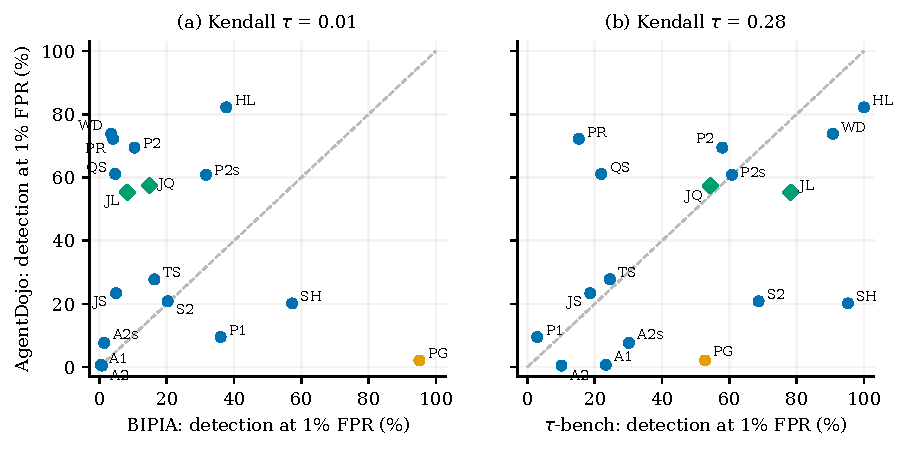
\includegraphics[width=0.85\textwidth]{figures/fig_rank.pdf}
\caption{Each point is a detector or judge (diamonds). (a) Detection on BIPIA does not predict detection on AgentDojo. (b) Detection on one agent benchmark predicts detection on the other only partly: Prismor (PR) and Sheltron (SH) trade places. Dashed line: equal performance. Key: HL Horizon-Labs, WD Wolf Defender, PR Prismor, P2/P2s Prompt Guard~2 86M/22M, P1 Prompt Guard~1, PG PIGuard, SH Sheltron, QS Qualifire Sentinel, S2 Sentinel v2, TS TestSavant, JS JasperLS, A1/A2/A2s ProtectAI v1/v2/v2-small, JQ/JL Qwen/Llama judge.}
\label{fig:rank}
\end{figure*}

\finding{2}{A detector's detection rank on one benchmark is a weak guide to its rank on another ($\tau$ between \RankTau and \TauBITB, none significant). The best detector on BIPIA catches \ADPGTpr of AgentDojo injections at 1\% FPR, and a detector that catches \MPRAD of AgentDojo injections catches \TBTprPR on $\tau$-bench.}

\subsection{RQ3: Training Data}
\label{sec:rq3}

Where training data is public, it explains the ranking, and it shows that what transfers is the form of the inputs, not the attack strings.

\paragraph{PIGuard and BIPIA.}
PIGuard's published training split contains \PGBipiaRows labeled BIPIA inputs: full emails, tables, and code answers with and without inserted attacks (median \PGBipiaChars characters). The verbatim overlap is large (Table~\ref{tab:overlap}): \OvTextTrain text attacks and \OvCodeTrain code attacks from BIPIA's training half appear, as do \OvCleanEmail of BIPIA's clean emails and \OvCleanCode of its clean code contexts. None of BIPIA's test-half attacks appear, and our main results use only those; restricting to them lowers PIGuard's detection at 1\% FPR only from \BISplitPGTrainTpr to \BISplitPGTestTpr, because the two halves come from the same generator and are inserted into the same kinds of content. Training on one half and testing on the other is standard practice; the result is an in-distribution score.

\paragraph{PIGuard and InjecAgent.}
PIGuard's training split also contains \NIASeen InjecAgent attack instructions, but in another form: \PGIARows short prompts (median \PGIAChars characters) that pair an attack with a generic task sentence, not attacks inside tool responses. This gives a controlled comparison within TB-Matched, where every injected output has the same form. PIGuard detects \TBSeenPG of the outputs carrying an attack it was trained on and \TBUnseenPG of those carrying one of the \NIAUnseen attacks it was not. Having seen the attack text does not help when the surrounding input is new.

\paragraph{Horizon-Labs and the agent benchmarks.}
Horizon-Labs uses BIPIA only for evaluation and removes evaluation texts from its training data. Its training set includes five public datasets of injections planted in documents and tool responses. Our audit of those five finds no BIPIA attack string, no AgentDojo attack template, and no InjecAgent instruction. It is nevertheless the best detector on both agent benchmarks; what it shares with them is the form of input, structured tool output with planted instructions.

\paragraph{The others.}
Wolf Defender's card reports evaluation on a benchmark built from AgentDojo's injection payloads; its training data is not public. Prismor was fine-tuned on two prompt-level injection datasets. AgentDojo's templates are explicit instructions addressed to the model (``ignore your previous instructions'', ``this is an important message''), which resemble direct prompt injections; InjecAgent's attacks inside $\tau$-bench product names and BIPIA's attacks inside emails and tables do not. Prismor detects the first and not the others.

\begin{table}[t]
\centering\small
\caption{Verbatim overlap between BIPIA and PIGuard's published training split (whitespace and case normalized). A lower bound: paraphrases are not counted.}
\label{tab:overlap}
\begin{tabular}{@{}lr@{}}
\toprule
BIPIA component & Found in training split \\
\midrule
Text attacks, training half & \OvTextTrain \\
Code attacks, training half & \OvCodeTrain \\
Text attacks, test half & \OvTextTest \\
Code attacks, test half & \OvCodeTest \\
Clean email contexts & \OvCleanEmail \\
Clean code contexts & \OvCleanCode \\
Clean table contexts & \OvCleanTable \\
AgentDojo attack templates & none \\
\bottomrule
\end{tabular}
\end{table}

\finding{3}{Detectors work on inputs whose form resembles their training inputs. PIGuard's BIPIA score rests on training on full BIPIA inputs; having seen InjecAgent's attack strings as short prompts does not help it detect them inside tool outputs (\TBSeenPG versus \TBUnseenPG). Horizon-Labs leads both agent benchmarks without any overlap, after training on agent-style inputs.}

\subsection{RQ4: Task Awareness and Attack Goals}
\label{sec:rq4}

\paragraph{Judges.}
Telling a general-purpose model the user's request makes it a reasonable detector: at 1\% FPR the Qwen judge catches \ADJQTpr of AD-Matched and \TBTprJQ of TB-Matched injections, and the Llama judge \ADJLTpr and \TBTprJLl. Llama-3.1-8B was trained on data from before AgentDojo existed, so its detection cannot come from memorizing AgentDojo. On both agent benchmarks the judges stay below the best dedicated detectors, at the cost of a 7--8B forward pass per tool output.

\paragraph{Task-aware Sheltron.}
Passing the user's request to Sheltron in a trusted segment raises its AUROC on AD-Matched from \MSHADAuc to \MSHTADAuc but lowers its detection at 1\% FPR from \MSHAD to \MSHTAD, and raises its false-positive rate on clean tool outputs from \MSHClean to \MSHTClean on AgentDojo and from \TBFPRSH to \TBFPRSHT on $\tau$-bench. This use is undocumented and may simply be out of distribution for the model.

\paragraph{Attack goals.}
Figure~\ref{fig:goal} breaks BIPIA's test-half injections into BIPIA's five official groups, each method at its own 1\%-FPR threshold on BIPIA. No approach other than the BIPIA-trained PIGuard covers all groups. Task-irrelevant injections, which ask the model to perform some unrelated harmless task, are the hardest: apart from PIGuard (\GPGIrr), the best approach is Prompt Guard~1 with \GPGoIrr, and every other approach catches at most \GSHIrr. The others split the remaining groups: Sheltron catches \GSHRel of task-relevant and \GSHTgt of targeted injections but \GSHAct of active code attacks, while the Qwen judge catches \GJQPas and \GJQAct of passive and active code attacks and \GJQRel of task-relevant ones. Our judge prompt asks about actions and tells the model not to flag ordinary requests between people; we did not vary it, so we cannot say how much of the judges' gap comes from the question we asked.

\begin{figure*}[t]
\centering
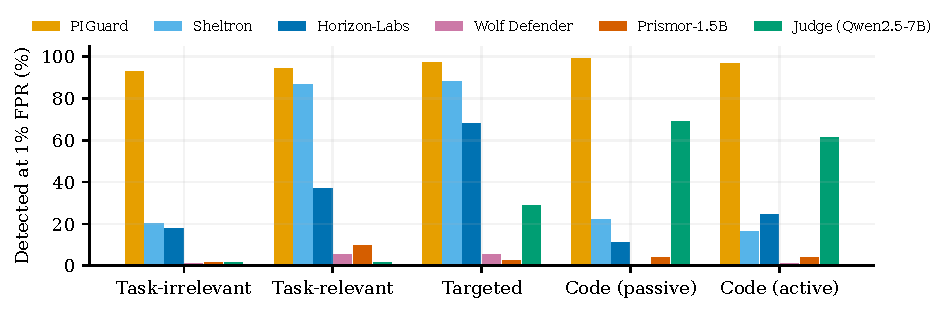
\includegraphics[width=0.92\textwidth]{figures/fig_goal_many.pdf}
\caption{Detection by BIPIA attack group (test half), each method at its own 1\%-FPR threshold on BIPIA. Only PIGuard, which was trained on BIPIA inputs, covers all groups; every other approach shown misses most task-irrelevant injections.}
\label{fig:goal}
\end{figure*}

\finding{4}{Task-aware 7--8B judges detect 54--78\% of injections in agent tool outputs at 1\% FPR, below the best dedicated detectors, and giving the user's request to a small classifier does not help. Outside its training distribution, every approach misses whole classes of injections, and task-irrelevant injections evade nearly all of them.}

\subsection{RQ5: Format and Metadata}
\label{sec:rq5}

How a tool output is presented to a detector moves its false-positive rate. README chunks that PIGuard flags are full of HTML tables, badges, and links rather than instructions; stripping markup lowers its FPR on READMEs from \FmtPGReadmeOrig to \FmtPGReadmePlain and ProtectAI v2's from \FmtPAReadmeOrig to \FmtPAReadmePlain (Figure~\ref{fig:format}). On AD-Matched, removing YAML keys so that PIGuard sees only values lowers its FPR from \ADPGFprHalf to \ADPGNFprHalf at the same TPR (\ADPGTprHalf versus \ADPGNTprHalf). Sheltron's source token has the largest effect: declaring a tool output as \texttt{tool\_result} instead of \texttt{other} lowers its FPR on clean tool outputs from \MSHGClean to \MSHClean on AgentDojo and from \TBFPRSHG to \TBFPRSH on $\tau$-bench.

These changes help less at the low-FPR end. With YAML keys removed, PIGuard catches \ADPGNTpr of AD-Matched injections at 1\% FPR and ProtectAI v2 \ADPANTpr. Sheltron with the specific source token catches \MSHAD on AD-Matched, compared with \MSHGAD with the generic one, and \TBTprSH versus \TBTprSHG on TB-Matched. Format and metadata shift a detector's scores; they do not make an out-of-distribution detector work.

\begin{figure}[t]
\centering
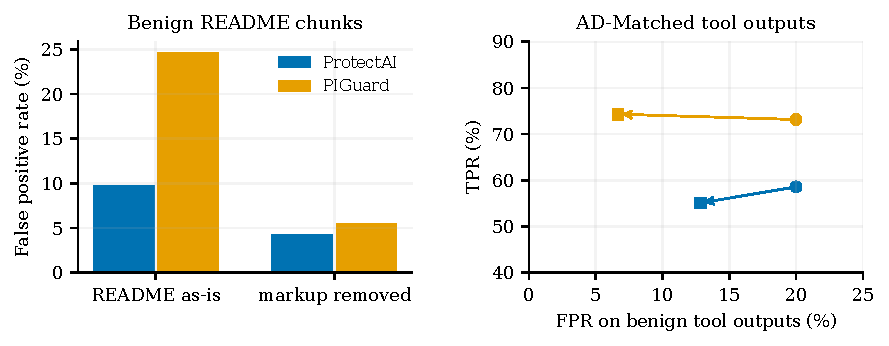
\includegraphics[width=\columnwidth]{figures/fig_format.pdf}
\caption{Format alone moves false positives. Left: removing markup from benign READMEs. Right: removing YAML keys from AgentDojo tool outputs (circle: as-is; square: keys removed) lowers PIGuard's FPR threefold at unchanged TPR.}
\label{fig:format}
\end{figure}

\finding{5}{Removing serialization markup or declaring the input type lowers default-threshold false positives by up to about twentyfold, a free improvement for deployments, but after any of these changes neither PIGuard nor ProtectAI v2 exceeds 15\% detection at 1\% FPR on AD-Matched.}
